\section{The number of SAC proteins recruited per signaling kinetochore depends on the total number of signaling kinetochores in the cell}

We then asked whether the differences between nocodazole- and GSK923295-treated groups were correlated with differential recruitment of these SAC proteins at signaling kinetochores and if so, whether these differences were contributed by \protein{Knl1} or the fibrous coronae (which is disrupted by \gene{ZW10} knockdown). Using wide-field fluorescence Microscopy, we determined that \protein{BubR1}, \protein{Bub1}, and \protein{Mad1} recruitment at signaling kinetochores are all enhanced when cells were treated with GSK923295 compared with nocodazole (\myref{SACProteinKinetochoreRecruitment_Quantification}).

\begin{figure}
    \centering
    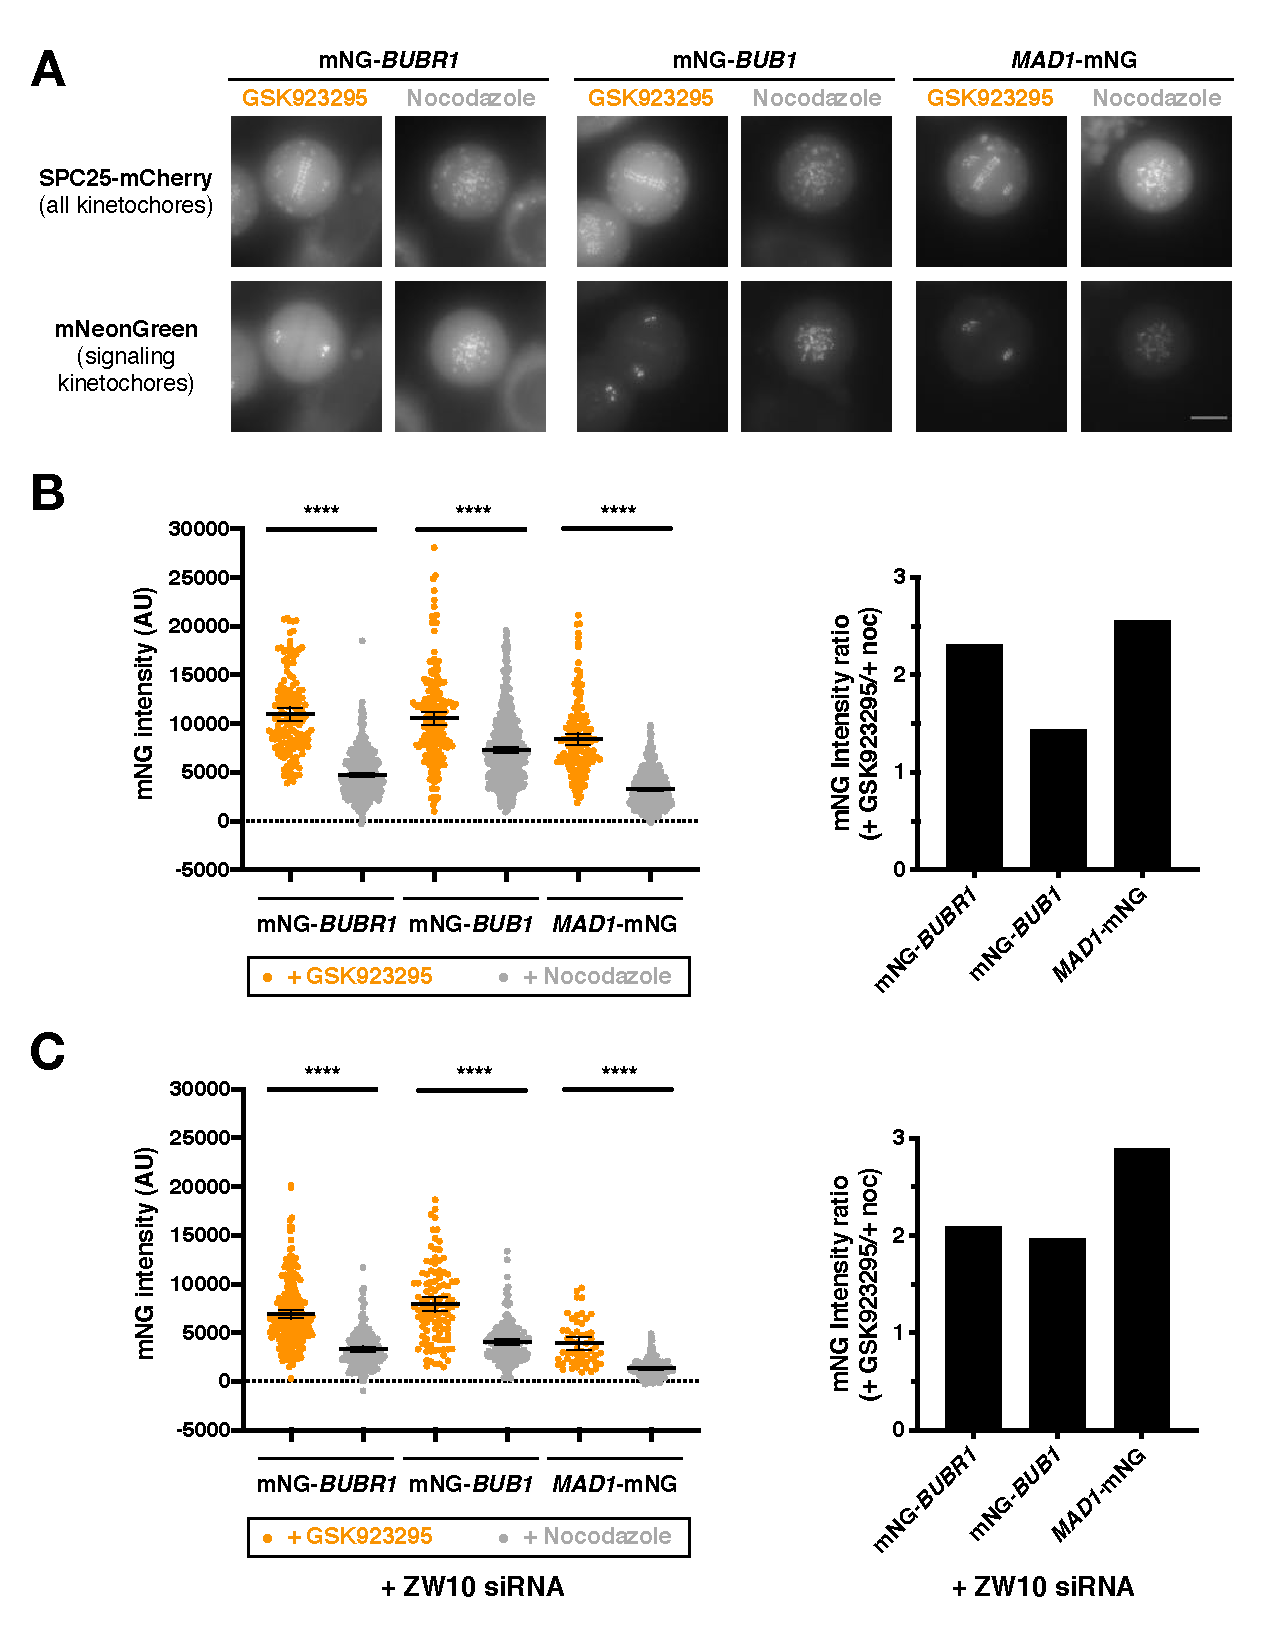
\includegraphics[width=\textwidth]{chapters/figures/SACProteinKinetochoreRecruitment.pdf}
    \phantomsubfiglabel{SACProteinKinetochoreRecruitment_Images} % subfigure A
    \phantomsubfiglabel{SACProteinKinetochoreRecruitment_Quantification} % subfigure B
    \phantomsubfiglabel{siZW10SACProteinKinetochoreRecruitment_Quantification} % subfigure C
    \caption{\textbf{\protein{BubR1} is more influential to SAC signaling strength and enriched at the few signaling kinetochores in GSK923295-treated cells than \gene{Bub1} and \protein{Mad1}.}}
    \noindent\justifying Lauren Humphrey-Stark performed all imaging and data analysis involved in this figure. \myref{SACProteinKinetochoreRecruitment_Quantification,siZW10SACProteinKinetochoreRecruitment_Quantification} were reproduced from one of my first-authored papers in preparation. (A) Mitotic duration (NEBD to anaphase onset) of HeLa-A12 cells with \Latin{in situ} mNeonGreen-tagged \gene{BubR1}, \gene{Bub1}, or \gene{Mad1} in the presence of 330 nM nocodazole or 236 nM GSK923295. Cells were transfected with either an mNeonGreen-targeting siRNA to knock down the corresponding SAC gene (left panel) or a negative control siRNA (right panel). (B) Exemplary micrographs showing cells from the three HeLa-A12 cell lines treated with nocodazole or GSK923295. Spc25-mCherry labeled all kinetochores. Scale bar, \SI{10}{\micro m}. (B) Quantification of mNeonGreen signals at individual signaling kinetochores from experiments illustrated in (B). Each dot represents the measurement from one signaling kinetochore. Error bars represent 95\% confidence intervals of the mean. Results from at least two independent experiments are shown. Pairwise ratios between the average mNeonGreen signals at individual signaling kinetochores of GSK923295-treated cells and nocodazole-treated cells in (C).
    % Bub1/BubR1 recruitment data with knockdown of the RZZ complex compared with those with no siRNA deviate greatly from Zhang et al., 2019
    
\label{SACProteinKinetochoreRecruitment}
\end{figure}



\section{The equilibrium between the activity of \protein{Mps1} and counteracting phosphatases at signaling kinetochore is the same in nocodazole- and GSK923295-treated HeLa-A12 cells}

The observed difference in the recruitment of SAC proteins on a per kinetochore basis in nocodazole- and GSK923295-treated cells may be partially attributed to a potential shifting of the degree of phosphorylation of MELT motifs, according to a previous study \cite{MPS1senor}. We repeated the assay from this study in the HeLa A12 cell line using a similar phosphorylation sensor to probe the equilibrium between the activity of kinases (mainly \protein{Mps1}) and counteracting phosphatases at the kinetochore (hereinafter referred to as \protein{Mps1}'s activity for simplicity). The only difference between our sensor and the original design of MPS1sen-KT is that we used mNeonGreen/mScarlet-I as the acceptor/donor combination, which suits our confocal microscopy setup.
%The expression cassette of the recombinant sensor is stably integrated into the genome via Cre-Lox recombination-mediated cassette exchange (\myref{Knl1RescueDesign}).
Since the acceptor and the donor has a fixed stoichiometry ($1 : 1$ in this case \ref{MPS1sen-KT_WB}),
%The majority of the recombinant protein detected by anti-DsRed2 antibody was the intact form. No major partial degradation products (like mScarlet-I-SPC24) was observed.
the ratio between the green channel readout and the raw FRET channel readout (even without corrections for the cross-excitation of the acceptor and the bleed-through of donor fluorescence) can be employed as a normalized measurement of the FRET efficiency (and therefore a normalized indicator of \protein{Mps1}'s activity).

We confirmed that sensors recruited to unaligned kinetochores in both nocodazole- and GSK923295-treated cells had lower FRET efficiencies (higher activities of \protein{Mps1}) compared to kinetochores aligned at metaphase plates in GSK923295-treated cells, consistent with the previous findings. However, in contrast to findings from \cite{MPS1senor}, we did not observe significantly different FRET efficiency of sensors recruited to unaligned kinetochores in nocodazole- and GSK923295-treated cells. This was irrelevant to the concentrations of respective drugs and the reason for the conflicting observations is unclear. As far as HeLa A12 (used throughout this study as the parental cell line) is concerned, no difference in \protein{Mps1}'s activity at unaligned kinetochores in nocodazole- and GSK923295-treated cells was detected. Therefore, the difference in the recruitment of SAC proteins on a per kinetochore basis in nocodazole- and GSK923295-treated cells should be mainly attributed to the difference in the number of signaling kinetochores competing for the limited pool of SAC protein based on the law of mass action.

It has been reported previously that the average localization levels of endogenously tagged HA-mCherry-\protein{Bub1} to signaling kinetochores in a CRISPR-Cas9-edited HeLa cell line treated with either \SI{250}{nM} of GSK923295 or \SI{6.6}{\micro M} of nocodazole were not significantly different \cite{MPS1senor}. One possible explanation is that the much higher concentration of nocodazole in the aforementioned study may contribute to a more complete breakdown of spindles and a higher number of phosphorylated MELT motifs, while the higher concentration of GSK923295 and the lack of filtering of cells based on the total number of unaligned chromosomes could mean more signaling kinetochores in GSK923295-treated cells.

\begin{figure}
    \centering
    \includegraphics[width=0.95\textwidth]{chapters/figures/MPS1sen-KT.pdf}
    \phantomsubfiglabel{MPS1sen-KT_Scheme} % subfigure A
    \phantomsubfiglabel{MPS1sen-KT_Images} % subfigure B
    \phantomsubfiglabel{MPS1sen-KT_FRETMetric} % subfigure C
    \caption{\textbf{No difference in the \protein{Mps1}-phosphatases equilibrium at signaling kinetochores was detected in HeLa A12 when cells were treated with different drugs at various concentrations.}}
    \noindent\justifying (A) The design scheme of MPS1sen-KT. The \protein{Mps1} substrate sequence is \Peptide{LLEDGTLAINW}. The only difference between our sensor and the original design \cite{MPS1senor} is that we replaced the donor/acceptor pair with mNeonGreen/mScarlet-I, which works better with our imaging setup. (B) Top panel: representative images of cells expressing MPS1sen-KT. MPS1sen-KT was recruited to both unaligned signaling kinetochores (in Nocodazole- and GSK923295-treated cells) and aligned non-signaling kinetochores (in GSK923295-treated cells) via its C-terminal \protein{Spc24} module. Brightness and contrast have been adjusted but the look-up table for each channel (row) is universal for different groups (column). Scale bar, \SI{10}{\micro m}. Bottom panel: using an antibody against DsRed2 (which can detect many RFPs including mScarlet-I), we confirmed that MPS1sen-KT (with a theoretical molecular weight of \SI{97.2}{kDa}) can be induced by doxycycline to express as a full-length protein with negligible partial degradation or cleavage products in the RMCE HeLa-A12 cells (right blot). A Ponceau S staining of the same blot before membrane blocking (left blot) serves as the loading control. (C) A summary of a normalized FRET metric (mNeonGreen signal/FRET signal) in HeLa A12 cells treated with different drugs at various concentrations. Each gray dot represents a single kinetochore measurement. Data were compiled from at least two independent experiments (more than 40 cells in total for each group). Mean values $\pm 95\%$ confidence intervals are overlaid. Data from cells treated with \SI{45}{nM}, \SI{90}{nM}, and \SI{200}{nM} GSK923295 were pooled together (they have no significant difference from one another) to simplify the presentation. The Welch's ANOVA test [$W(\text{DF}n, \text{DF}d) = 1.339 (2.000, 917.0)$, $P = 0.2626$] was performed for the first 3 columns (signaling kinetochores). The unpaired $t$-test with Welch's correction ($P < 0.0001$) was performed to compare aligned non-signaling kinetochores with unaligned signaling kinetochores in GSK923295-treated cells. Statistical tests were done in Prism 9.
    \label{MPS1sen-KT}
\end{figure}









Unattached kinetochores catalyze MCC formation by recruiting SAC proteins in a well-defined signaling cascade (Fig. 1A) (Faesen et al., 2017; Ji et al., 2017; Lara-Gonzalez et al., 2021a; London and Biggins, 2014; London et al., 2012; Piano et al., 2021; Primorac et al., 2013; Shepperd et al., 2012). This cascade is activated when the kinetochore protein Knl1 is phosphorylated by the Mps1 kinase at the ‘MELT’ motifs, so called because of their consensus amino acid sequence in humans and other eukaryotes (Primorac et al., 2013; Tromer et al., 2015; Vleugel et al., 2013). Each MELT motif serves as the scaffold for recruiting downstream signaling proteins (Chen et al., 2019; Primorac et al., 2013). Prior studies in human cells have shown that the strength of the SAC is weakly correlated with the number of MELT motifs in KNL1 and the amount of SAC proteins that they recruit (Vleugel et al., 2015; Vleugel et al., 2013; Zhang et al., 2014). The cumulative amount of MCC generated by the kinetochores is also weakly correlated with the number of signaling kinetochores (Collin et al., 2013; Dick and Gerlich, 2013). To understand why, we decided to quantify the copy number of SAC proteins recruited by individual signaling kinetochores to assess their steady state signaling activity. We focused on one protein each from the three layers of the recruitment cascade: Bub1, BubR1, and Mad1. We selected Bub1 because it recruits BubR1, the Mad1-Mad2 complex, and Cdc20 (Lara-Gonzalez et al., 2021a; Piano et al., 2021), BubR1 because it is an essential MCC component, and Mad1 because it helps catalyze the conformational change in Mad2 necessary for forming the MCC (Mapelli et al., 2007). 
To ensure accurate quantification and comparative analysis, we used genome-edited HeLa cells that express either mNeonGreen-Bub1, mNeonGreen-BubR1, or Mad1-mNeonGreen [“mNeonGreen” is abbreviated as “mNG” henceforth; (Shaner et al., 2013)]. In these cells, about half of the total protein is fluorescently labeled; the remaining protein is unlabeled (Banerjee et al., 2021). Because the fluorescent tags are separated from the tagged proteins by flexible linkers, we assume that they do not interfere with protein recruitment or function. With this assumption, we expect signaling kinetochores to recruit roughly equal amounts of labeled and unlabeled proteins. 
Our goal was to characterize the dependence of Bub1, BubR1, and Mad1 recruitment per kinetochore on the number of signaling kinetochores in the cell. To attain it, we obtain mitotically arrested cells containing distinctly different numbers of signaling kinetochores using two drugs. To obtain cells with nearly all kinetochores unattached, we released G1/S arrested HeLa cells into the cell cycle and then arrested them in mitosis using 330 nM nocodazole, a drug that depolymerizes microtubules (Figure 1B, right). These cells serve as a model for prophase cells. To obtain mitotic cells with a much smaller number of signaling kinetochores, we released G1/S arrested HeLa cells into the cell cycle and treated them with 236 nM GSK923295, a small molecule inhibitor of the mitotic kinesin CENP-E one hour prior to imaging (Qian et al., 2010). In these cells, a variable, but smaller, number of chromosomes stranded at the spindle poles with kinetochores (Figure 1B, left). These kinetochores are either unattached or laterally attached, and they activate the SAC by recruiting SAC signaling proteins (Krefman et al., 2015; Kuhn and Dumont, 2019). The remaining chromosomes align at the metaphase plate, and their kinetochores recruit significantly lower amounts of SAC proteins. These cells serve as the model for prometaphase cells. Because the number of signaling kinetochores is variable in GSK923295-treated cells, we analyzed only those cells that contained ~ 10 polar chromosomes or less based on a visual inspection of the image stacks. To estimate the number of molecules per kinetochore from the measured mNG signal per kinetochore, we also imaged HeLa cells exogenously expressing Spc25-mNG under identical imaging conditions. Spc25 is a subunit of the Ndc80 complex, and it is known that: (a) the human kinetochore contains ~ 250 molecules of the Ndc80 complex and (b) the stoichiometry between Ndc80 and Knl1 is 3:2 (Suzuki et al., 2015). This information allowed us to estimate the number of each SAC protein per Knl1 and thus relate it to the number of MELT motifs per Knl1.
We first examined SAC protein recruitment in cells treated with nocodazole. Using the calibration standard above, we estimate that in cells containing many signaling kinetochores each Knl1 molecule recruits only 2.3 ± 1.1 Bub1 molecules (mean ± std. dev.). This number is lower than the previously reported value of ~ 4-6, possibly because expression level of exogenous, labeled Bub1 may have been higher than physiological levels (Vleugel et al., 2015). BubR1 and Mad1 recruitment per kinetochore in nocodazole-treated cells was lower than the Bub1 recruitment (1.5 ± 0.9 and 1 ± 0.9 molecule per Knl1, respectively). Given that Knl1 contains 19 putative MELT motifs with different affinities for binding Bub1-Bub3, these results show that, each kinetochore uses only a fraction of its maximal signaling capacity under the experimental conditions (Vleugel et al., 2015). Similar observations were also made in budding yeast (Aravamudhan et al., 2016).
We next quantified the recruitment of the three SAC proteins in GSK923295-treated cells containing far fewer signaling kinetochores (Figure 1B). In these cells, the recruitment per kinetochore was significantly higher for all three proteins. The number of Bub1 molecules per kinetochore increased to 3.3 ± 1.5; the number of BubR1 and Mad1 molecules per kinetochore was equal to Bub1 (3.5 ± 1.3 and 2.7 ± 1.2 per kinetochore, respectively). Taken together with the data from nocodazole-treated cells, these measurements suggest that the number of SAC proteins recruited per kinetochore is inversely correlated with the number of signaling kinetochores in the cell. This trend is consistent with observations made in budding yeast (Aravamudhan et al., 2016). 
It should be noted that Mad1-Mad2 is recruited to metazoan kinetochores by Bub1 as well as the RZZ complex (Pereira et al., 2018; Rodriguez-Rodriguez et al., 2018; Silio et al., 2015). To quantify the fraction of Mad1-Mad2 recruited by RZZ, we depleted the Zw10 subunit of the RZZ complex using RNA interference (RNAi) in the three cell lines (Methods) and then quantified the recruitment of the mNG-labeled SAC proteins to signaling kinetochores as before. ZW10 siRNA treatment resulted in a ~ 25% decrease in Bub1 and BubR1 recruitment, as noted by others (Kops et al., 2005). As expected, Mad1 recruitment was significantly lower in both GSK923295 and nocodazole-treated cells (Figure S1). The number of Mad1 molecules recruited per Bub1 molecule was reduced by ~ 50% revealing the contribution of the RZZ under these conditions. The number of Bub1 and BubR1 molecules per kinetochore was also reduced; however, the two proteins were recruited in approximately equal amounts.

Mps1-mediated phosphorylation within signaling kinetochores is the same in nocodazole- and GSK923295-treated cells
The observed difference in the recruitment of SAC proteins on a per kinetochore basis in nocodazole- and GSK923295-treated cells may be due to a shift of the degree of phosphorylation of MELT motifs. To test this hypothesis, we quantified the net Mps1-mediated phosphorylation within the kinetochore using a recently developed FRET-based sensor of Mps1 kinase activity that was fused to the N-terminus of the kinetochore subunit Spc24 (Kuijt et al., 2020). We modified this sensor to use mNeonGreen/mScarlet-I as the acceptor/donor combination (Figure 2A-B). Since the acceptor and the donor has a fixed 1:1 stoichiometry in the sensor, we used the ratio of the green channel readout and the raw FRET channel readout (without corrections for the cross-excitation of the acceptor and the bleed-through of donor fluorescence) as the normalized measurement of the FRET efficiency and the net Mps1-mediated phosphorylation. 
We confirmed that Mps1-sensor recruited to unaligned kinetochores in both nocodazole- and GSK923295- treated cells had lower FRET efficiencies (higher activities of Mps1) compared to kinetochores aligned at metaphase plates in GSK923295-treated cells (Figure S2). Importantly, we did not detect any difference in the net Mps1-mediated phosphorylation within unaligned kinetochores in nocodazole- and GSK923295-treated cells irrespective of the drug concentration used. Therefore, the difference in the recruitment of SAC proteins on a per kinetochore basis in nocodazole- and GSK923295-treated cells should be mainly attributed to competition for the limited pool of SAC protein based on the law of mass action. This observation contrasts with the previous report that the average localization levels of endogenously tagged HA-mCherry-Bub1 to signaling kinetochores in a CRISPR-Cas9-edited HeLa cell line treated with either 250 nM of GSK923295 or 6.6 μM of nocodazole were not significantly different (Kuijt et al., 2020). One possible explanation is that the much higher concentration of nocodazole in the aforementioned study may contribute to a more complete breakdown of spindles and a higher degree of phosphorylation of MELT motifs, while the lack of filtering of GSK923295-treated cells based on the number of unaligned chromosomes would lead to similar average numbers of signaling kinetochores in the Nocodazole- and GSK923295-treated cells. We also cannot rule out the possibility that the differences reflect different Bub1 expression levels or kinase/phosphatase activities in the HeLa cell lines used.
